%
% einleitung.tex -- Beispiel-File für die Einleitung
%
% (c) 2020 Prof Dr Andreas Müller, Hochschule Rapperswil
%
\section{Motivation\label{transfer:section:teil0}}
\rhead{Einleitung}

Die Transferfunktion ist einer der wichtigsten Bestandteile moderner
neuronaler Netzwerke.
\index{Transferfunktion}%
\index{neuronales Netzwerk}%
Sie verleiht ihnen die Nichtlinearität, welche
\index{Nichtlinearität}%
benötigt wird, um komplexere Aufgaben zu lösen.
Dabei kann theoretisch jede nichtlineare Funktion eingesetzt werden.
In der Praxis tauchen
aber nur sehr wenige Funktionen mit ähnlichen Eigenschaften auf.
Einige davon sind in der Tabelle \ref{tab:aktfkt} zu sehen.
In der
heutigen Zeit sind vor allem die Variationen der ReLU Funktion
beliebt.
Dies vor allem wegen der einfachen Berechnung.
Der Tangens hyperbolicus wird aber dank dem Aufkommen der Recurrent
Neural Networks, zum Beispiel dem Long short-term memory Netzwerk,
das aus Zellen wie in Abbildung \ref{motivation:figure:LSTM} gezeigt
bestehen, wieder vermehrt eingesetzt.
Die klassische Berechnung, welche in Abbildung
\ref{anleitung:figure:approxtanhhypalgo} gezeigt wird, ist aber
sehr aufwendig und basiert auf Gleitkommaoperationen und relativ
\index{Gleitkommaoperationen}
komplizierten Funktionen. Diese benötigen einen grossen Rechenaufwand
vor allem auf Systemen die keine Gleitkommaarithmetikhardware
besitzen wie das zum Beispiel bei gewissen Mikrocontrollern der
\index{Mikrocontroller}
Fall ist.

Es gibt verschiedene Ideen diese Berechnung durch Approximationsalgorithmen
zu vereinfachen. Basierend auf der Arbeit von Abhisek Kundu et al.
(2019) \cite{transfer:DBLP:journals/corr/abs-1909-07729} werden
hier beliebte Algorithmen aufgezeigt und verglichen.

\tikzset{font={\fontsize{10pt}{12}\selectfont}}
\begin{table}[h]
	\centering
	\begin{tabular}{llll}
		\hline
		\multicolumn{1}{l}{Name} & \multicolumn{1}{l}{Funktion} & \multicolumn{1}{l}{Graph} \\ 
		\hline
		Sigmoid & $\sigma(x)=\frac{1}{1+e^{-x}}$ & 
		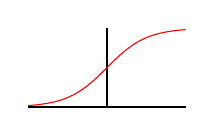
\begin{tikzpicture}[baseline={(0,0.2)}]
			\draw (-1,0) -- (1,0);
			\draw (0,0) -- (0,1);
			\draw[red] plot[domain=-1:1,variable=\x] ({\x},{1/(1+exp(-4*\x))});
		\end{tikzpicture}\\
		ReLU & $f(x) =\begin{cases}
			0 & ~\text{für}~ x<0 \\ 
			x & ~\text{für}~x \geq 0.
		\end{cases}$ &
		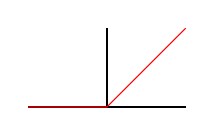
\begin{tikzpicture}[baseline={(0,0.5)}]
			\draw (-1,0) -- (1,0);
			\draw (0,0) -- (0,1);
			\draw[red] plot[domain=-1:1,variable=\x] ({\x},{ifthenelse(\x<0,0,\x)});
		\end{tikzpicture}\\
		Leaky ReLU & $f(x) =\begin{cases}
			0 & ~\text{für}~ x<0 \\ 
			x & ~\text{für}~x \geq a \cdot x.
		\end{cases}$ &
		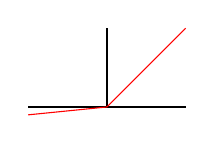
\begin{tikzpicture}[baseline={(0,0.5)}]
			\draw (-1,0) -- (1,0);
			\draw (0,0) -- (0,1);
			\draw[red] plot[domain=-1:1,variable=\x] ({\x},{ifthenelse(\x<0,0.1*\x,\x)});
		\end{tikzpicture}                            
	\end{tabular}
	\caption{Transferfunktionen}
	\label{tab:aktfkt}
\end{table}

\begin{figure}
\centering
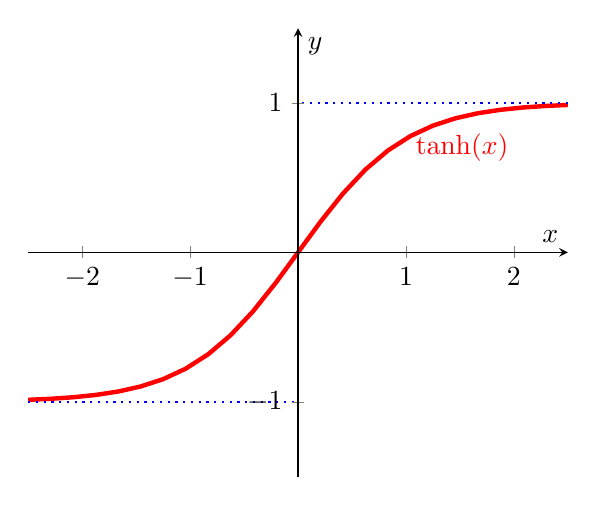
\begin{tikzpicture}
	\begin{axis}[
		xmin=-2.5, xmax=2.5,
		ymin=-1.5, ymax=1.5,
		axis lines=center,
		axis on top=true,
		domain=-2.5:2.5,
		ylabel=$y$,
		xlabel=$x$,
		]
		
		\addplot [mark=none,draw=red,ultra thick] {tanh(\x)};
		\node [right, red] at (axis cs: 1,0.7) {$\tanh(x)$};
		
		%% Add the asymptotes
		\draw [blue, dotted, thick] (axis cs:-2.5,-1)-- (axis cs:0,-1);
		\draw [blue, dotted, thick] (axis cs:+2.5,+1)-- (axis cs:0,+1);
	\end{axis}
\end{tikzpicture}
\caption{Tangens hyperbolicus
\label{anleitung:figure:tanhyp}}
\end{figure}

\begin{figure}
\centering
\tikzset{
	decision/.style={
		shape=rectangle,
		minimum height=1cm,
		text centered,
		rounded corners=1ex,
		draw,
		label={[yshift=0.2cm]left:ja},
		label={[yshift=0.2cm]right:nein},
	},
	outcome/.style={
		shape=ellipse,
		fill=gray!15,
		draw,
		text centered
	},
	decision tree/.style={
		edge from parent path={[-latex] (\tikzparentnode) -| (\tikzchildnode)},
		sibling distance=4cm,
		level distance=1.5cm
	}
}

\begin{tikzpicture}
	
	\node [decision] { $x>k \cdot \frac{\ln 10}{2}$ }
	[decision tree]
	child { node [outcome] { $+1$ } }
	child { node [decision] { $x<-k \cdot \frac{\ln 10}{2}$} 
		child { node [outcome] { $-1$ } }
		child { node [decision] { $-0,1<x<+0,1$ } 
			child { node [outcome] { $\frac{\sinh x}{e^{x}-\sinh x}$ } }
			child { node [outcome] { $\frac{e^{2 x}-1}{e^{2 x}+1}$ } }
		}
	};
\end{tikzpicture}
\caption{Annäherung für Tangens hyperbolicus
\label{anleitung:figure:approxtanhhypalgo}}
\end{figure}


\begin{figure}
	\centering
	\newcommand{\empt}[2]{$#1^{\langle #2 \rangle}$}
	
	\begin{tikzpicture}[
		% GLOBAL CFG
		font=\sf,
		>=LaTeX,
		% Styles
		cell/.style={% For the main box
			rectangle,
			rounded corners=5mm,
			draw,
			very thick,
		},
		operator/.style={%For operators like +  and  x
			circle,
			draw,
			inner sep=-0.5pt,
			minimum height =.2cm,
		},
		function/.style={%For functions
			ellipse,
			draw,
			inner sep=1pt
		},
		ct/.style={% For external inputs and outputs
			circle,
			draw,
			line width = .75pt,
			minimum width=1cm,
			inner sep=1pt,
		},
		gt/.style={% For internal inputs
			rectangle,
			draw,
			minimum width=4mm,
			minimum height=3mm,
			inner sep=1pt
		},
		mylabel/.style={% something new that I have learned
			font=\scriptsize\sffamily
		},
		ArrowC1/.style={% Arrows with rounded corners
			rounded corners=.25cm,
			thick,
		},
		ArrowC2/.style={% Arrows with big rounded corners
			rounded corners=.5cm,
			thick,
		},
		]
		
		%Start drawing the thing...
		% Draw the cell:
		\node [cell, minimum height =4cm, minimum width=6cm] (cell) at (0,0){} ;
		
		% Draw inputs named ibox#
		\node [gt] (ibox1) at (-2,-0.75) {$\sigma$};
		\node [gt] (ibox2) at (-1.5,-0.75) {$\sigma$};
		\node [function, draw=red!60, fill=red!5] (ibox3) at (-0.5,-0.75) {$\tanh$};
		\node [gt] (ibox4) at (0.5,-0.75) {$\sigma$};
		
		% Draw op�rators   named mux# , add# and func#
		\node [operator] (mux1) at (-2,1.5) {$\times$};
		\node [operator] (add1) at (-0.5,1.5) {+};
		\node [operator] (mux2) at (-0.5,0) {$\times$};
		\node [operator] (mux3) at (1.5,0) {$\times$};
		\node [function, draw=red!60, fill=red!5] (func1) at (1.5,0.75) {$\tanh$};
		
		% Draw External inputs named as basis c,h,x
		\node[ct, label={[mylabel]}] (c) at (-4,1.5) {\empt{c}{t-1}};
		\node[ct, label={[mylabel]}] (h) at (-4,-1.5) {\empt{h}{t-1}};
		\node[ct, label={[mylabel]}] (x) at (-2.5,-3) {\empt{x}{t}};
		
		% Draw External outputs? named as basis c2,h2,x2
		\node[ct, label={[mylabel]}] (c2) at (4,1.5) {\empt{c}{t}};
		\node[ct, label={[mylabel]}] (h2) at (4,-1.5) {\empt{h}{t}};
		\node[ct, label={[mylabel]}] (x2) at (2.5,3) {\empt{h}{t}};
		
		% Start connecting all.
		%Intersections and displacements are used.
		% Drawing arrows
		\coordinate (e) at (cell.west |- c);
		\draw [->, ArrowC1] (c) -- (e);
		\draw [->, ArrowC1] (e) -- (mux1) -- (add1) -- (c2);
		
		% Inputs
		\coordinate (e) at (cell.west |- h);
		\draw [->, ArrowC2] (h) -- (e);
		\draw [ArrowC2] (e) -| (ibox4);
		\draw [ArrowC1] (h -| ibox1)++(-0.5,0) -| (ibox1);
		\draw [ArrowC1] (h -| ibox2)++(-0.5,0) -| (ibox2);
		\draw [ArrowC1] (h -| ibox3)++(-0.5,0) -| (ibox3);
		\coordinate (e) at (cell.south -| x);
		\draw [->, ArrowC1] (x) -- (e);
		\draw [ArrowC1] (e) -- (x |- h)-| (ibox3);
		
		% Internal
		\draw [->, ArrowC2] (ibox1) -- (mux1);
		\draw [->, ArrowC2] (ibox2) |- (mux2);
		\draw [->, ArrowC2] (ibox3) -- (mux2);
		\draw [->, ArrowC2] (ibox4) |- (mux3);
		\draw [->, ArrowC2] (mux2) -- (add1);
		\draw [->, ArrowC1] (add1 -| func1)++(-0.5,0) -| (func1);
		\draw [->, ArrowC2] (func1) -- (mux3);
		
		%Outputs
		\draw [->, ArrowC2] (mux3) |- (h2);
		\draw (c2 -| x2) ++(0,-0.1) coordinate (i1);
		\draw [-, ArrowC2] (h2 -| x2)++(-0.5,0) -| (i1);
		\draw [->, ArrowC2] (i1)++(0,0.2) -- (x2.south);
		
	\end{tikzpicture}
	\caption{Long short-term memory cell mit \empt{x}{t} als Input und \empt{h}{t} als momentaner Zustand, also Output. \empt{c}{t} fungiert als interner Zustand, der weitergegeben wird. Im inneren werden durch die Sigmoid-Layer und den Tangens hyperbolicus die Einflüsse der verschiedenen Eingänge und die neuen Zustände berechnet.
		\label{motivation:figure:LSTM}}
\end{figure}





